% This is LLNCS.DEM the demonstration file of
% the LaTeX macro package from Springer-Verlag
% for Lecture Notes in Computer Science, version 1.


%% \usepackage[T1]{fontenc}
%% \usepackage[latin9]{inputenc}
%% \usepackage{geometry}
%% \geometry{verbose,letterpaper,tmargin=5cm,bmargin=3cm,lmargin=3cm,rmargin=3cm,headheight=5cm,headsep=1cm}
%% \pagestyle{headings}
%% \usepackage{array}
%% \usepackage{verbatim}
%% \usepackage{longtable}
%% \usepackage{varioref}
%% \usepackage{float}
%% \usepackage{amsmath}
%% \usepackage{color} %%^^&&&&&&**** +++
%% \usepackage{graphicx}
%% \usepackage{amssymb}
%tzuf3110

\documentstyle[graphicx,amsmath,float,array]{llncs}

%
\begin{document}

\title{Parallel Transductive Linear SVM for Text Categorization}

\author{Miguel Fernando Cabrera and Jairo Espinosa Oviedo}

\institute{Universidad Nacional de Colombia - Sede Medell\'{i}n,
  Medell\'{i}n, Colombia
  {\it \{mfcabrer,jespinov\}}@unal.edu.co 
}


\maketitle

\begin{abstract}
Transductive Support Vector Machines (TSVM) have shown improvements
on classification tasks such as Text Categorization (TC), where the
features present co-occurrence and the training samples are few in
comparison with the data available. Although the nature of the TSVM
algorithm as described by Joachim makes it difficult to be as fast
as a regular SVM, the parallelization of this algorithm is interesting
when the gains in classification performance are crucial. Solving
TSVM algorithm requires the solution of multiple quadratic programming
problems that generally scales to $O(n^{3})$. We describe the implementation
of a TSVM Solver for 2-class problem using a parallel architecture
which aims to improve the necessary computation times while preserving
the classification performance. This strategy produced an implementation 
that is 2x - 7x faster than a regular TSVM for a TC problem of 2,000 vectors 
and more than 30,000 features.

{\bf Keywords:} SVM, Text Classification, Machine Learning, Algorithm,
Parallel Algorithm, Information Retrieval,Artificial Intelligence

\end{abstract}

\section{Introduction}

Text classification is a key aspect of text filtering, document management
and retrieval tasks. Besides basic document classification many problems can be seen as instances of
a Text Categorization (TC) problem. Spam detection, Web search
improvement and automated metadata generation are just a few examples
of this \cite{Sebastiani02}.  Some of those tasks can be achieved
by human beings, but a manual classification is at best expensive
and practically impossible for large amounts of documents found today
in modern information systems.

%% A TC technique uses example documents that have been previously categorized
%% in classes by an authority in order to learn a model that, with an
%% associated error value, can automatically predict the class that the
%% authority would have given to future documents. 

Support Vector Machines \cite{Vapnik98} are powerful tools for classifying
large data sets, and due the nature of the classical text representation
models, it has been applied successfully in automated document classification
tasks \cite{Joachims98,Joachims99c}. An special type of SVM, based
on Transductive inference (TSVM), has demonstrated to be more effective
for document classification than the common inductive inference based
SVM \cite{Joachims99c}.

One characteristic of the SVM is that, in its formal definition, the
computation and memory storage requirements increase rapidly with
the number of training vectors. This is due the fact that the SVM
classification problem is a Quadratic Programming problem (QP) that
finds the support vectors in all training data set. Solvers of this
kind of problem generally scales to $O(n^{3})$ making it a very computationally
expensive problem.

%% One approach to cope with this limitation is to divide the problem
%% into chunks \cite{Joachims/99a,osunaetal97} and train those sub-problems.
%% Even with these optimizations, the problem still has large computational
%% requirements, and the required time to train grows sufficiently enough
%% for making it not useful for real-time training when using large data
%% sets. The implementation of Transductive inference for a SVM requires
%% to solve the same problem many times over generally large data sets,
%% until finding the optimal classifier. This makes the scaling problem
%% for Transductive SVM even more difficult, therefore, methods for optimizing
%% the training process need to be developed.

%% Taking advantage actual trends in processor technologies, where the
%% multi-core processor is becoming the norm \cite{Marowka07,1069628|Geer05}
%% parallel implementation of such algorithm along with other optimization
%% will help make the application of this technique practical in real
%% world situations. Also, as an extra motivation, empirical results
%% have showed that some parallel settings for SVM have achieved better
%% generalization than their classic counterparts for some problems \cite{citeulike:935557|Collobert2002}.

This paper describes an implementation of a parallel SVM with the
cascade model described in \cite{GrafCBDV04} using a Transductive
learning algorithm. 
%% The first part, Overview, introduces the basic
%% concepts a Machine Learning, Information Retrieval and Text Categorization.
%% Later we describe the SVM algorithm and justify the reason of using
%% SVM for text classification over other techniques. In chapter \ref{cha:Experiments-and-Results}
%% we exhibit our experimental set-up and the show the analysis of the
%% results.

%
\section{Models of Text and Text Representation\label{sub:Models-of-Text}}
%

Usually in a digital library database a set of words that defines
the topics or the main characteristics of a document is manually defined.
The main objective of this is to help the search of the physical document
(e.g books, papers,etc.). This list of terms or keywords enables the
user to query documents related to one or more concepts. One of the
main problems of this is that only few keywords are associated with
a defined document, and generally this assignation is made at hand,
making it expensive and error prone.
%%% Generally this querying these
%% systems was limited to the numbers of keywords assigned and some metadata
%% like title, author and dates of publication, being the user unable
%% to query the whole document, making the retrieval task significantly
%% harder.
%% Nowadays digital libraries and similar systems where the all the
%% text is available in digital form, automatic keyword extraction makes
%% sense because these keywords are tightly associated with the content.
%% This keywords are called indexes and the task of associating each
%% document with a set of keywords is called \emph{indexing}. 
%% Indexing is based is predefined group of keywords: the dictionary
%% or vocabulary. As mentioned above, in a digitalized text database 
%% (also called a corpus) the dictionary is usually extracted from the
%% set of words present in the corpus, and the expensive manual indexing
%% can be avoided by representing the documents by the dictionary terms
%% they are made of. Given that all the full text is available for querying
%% it, now problem is to find the best way of representing the text in
%% order to extract the more important words, that is, the keywords that
%% define it. 

During the last few decades many representation forms have been developed
ranging from simple word appearance binary representation to a concept
\cite{deerwester90indexing}, probabilistic and
even Neural Networks \cite{DBLP:conf/icann/KellerB05} based ones. 
%% \cite{keller-theme} \cite{361220}

The most common approach to automatically extract the index terms
from a corpus is called vector space model. In this
model each document $d$ is represents as a vector$(\theta_{1},...,\theta_{M})$
where $\theta_{j}$ is a function of the frequency in $d$ of the
$j^{th}$ word of a chosen dictionary $M$. 

Based in this definition various forms of $\theta(j)$have been defined,
however the most popular ones are the variations of [{\emph{tf-idf}}]  In
which $\theta_{j}$ is equal to the formula:
\begin{equation}
\theta_{j}=tf_{j}(d)\centerdot log(\frac{N}{df_{j}}),\,\,\,\,\forall j\in\{1,\ldots,M\}\label{eq:tf-idf}\end{equation}

%% \begin{description}
%% \item [{Binary}] In which $\theta_{j}$ is equal to 1 if the $j^{th}$
%% word appears in the document or 0 otherwise.
%% \item [{Frequency}] In which $\theta_{j}$ is equal to the number of times
%% $j^{th}$ word appears in the document.
%% \item [{\emph{tf-idf}}] In which $\theta_{j}$ is equal to the \emph{tf-idf}
%% formula:
%% \end{description}
%% The equation \ref{eq:tf-idf} was defined proposed by Salton and Buckley
%% \cite{866292}. 
The $tf_{j}(d)$ (term frequency) is the number of times that the $j^{th}$ word appears
in the document $d$, $df_{j}$ is the number of documents the term
appears in all the corpus and $N$ is the total number of documents
in the corpus. 
%% The main reason behind this formulation is that in
%% the context of document retrieval it is considered that words appearing
%% too frequently across the corpus may not be discriminant, therefore
%% this formula gives more importance to terms appearing more frequently
%% in the documents while penalizing the ones that appears in to many
%% documents. The reader may have noticed that this representation of
%% text does not take into account the actual order of the words inside
%% the document, despite this, vector space model have performed well
%% and it still used with some variations in the majority of IR systems.

%% the vector space model representation described above may seem simplistic
%% in comparison with the more complex representations mentioned first,
%% nevertheless, it seems that for some tasks like text categorization,
%% the classical tf-idf works just well while more complex representations
%% of the text do not significantly affect the performance of the methods.

%
%% \Begin{figure}
%% \begin{centering}
%% 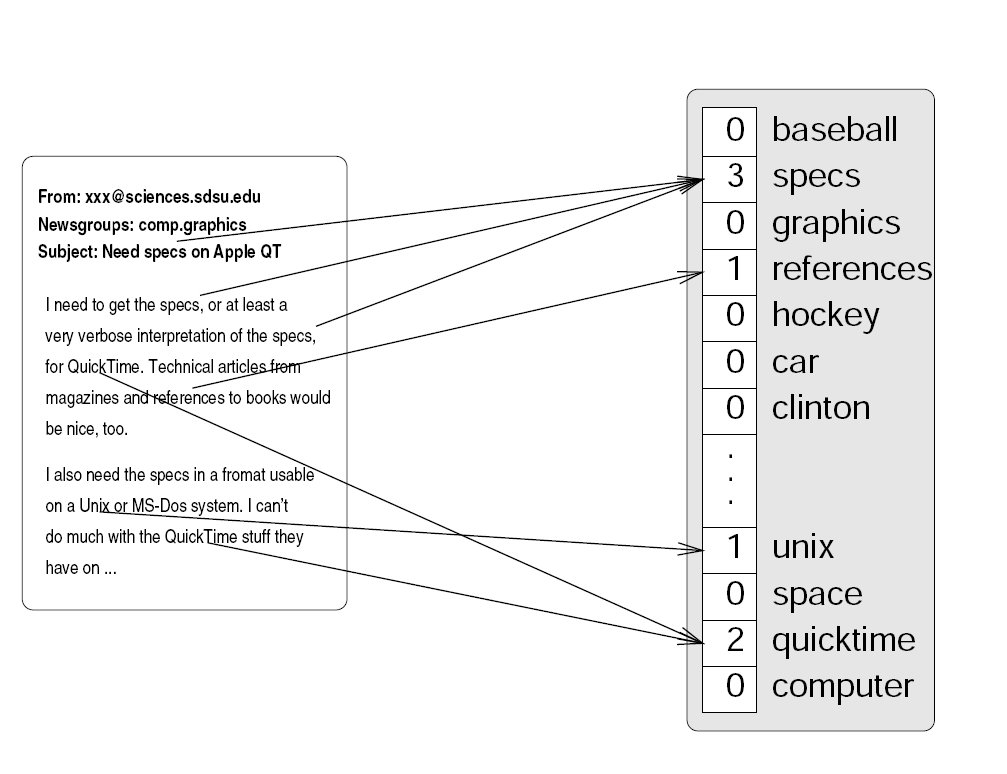
\includegraphics[scale=0.2]{images/joachims-text-vect}
%% \par\end{centering}

%% \caption{Representing text as a feature vector \cite{Joachims98}}

%% \end{figure}


\section{Support Vector Machines}

Support Vector Machines (SVMs) \cite{Vapnik98} are powerful classification
and regression tools that have been widely applied in the solutions
of many problem, generally yielding comparable or even better performance
that other algorithms. 

The SVM algorithm is based on the concept of VC Dimension\cite{vapnik71uniform}
and on the principle of structural risk minimization developed by
Vapnik \cite{Vapnik99,vapnik71uniform}. Roughly, the VC dimension
is a metric of how complex a classifier machine is, complex classifier
has more capacity to fit the training data, thus, overfitting is more
likely to occur, therefore, is preferred a classifier with minimum
VC Dimension. 

The basic idea of empirical risk minimization principle is to find
an hypothesis $s$ from an hypothesis space $S$ for which the lowest
probability of error is guaranteed for a given set of training examples. 
%% For linear classification problems this is equivalent to find the
%% discrimination function that maximizes the distances within the classes,
%% assuring the lowest probability of error\cite{citeulike:368926|Haykin1998}.
%% The aim of the Support Vector classification is to devise a computationally
%% efficient way of learning the optimal separating hyperplanes in high
%% dimensional feature space \cite{citeulike:114719|Cristianini2000introSVM}.

\section{SVM and Text Categorization}

The usage of SVM for TC  was first introduced by Joachims \cite{Joachims98,Joachims99c}
and similar setups have been used in posterior literature \cite{DumaisPHS98}.
the TC task using SVM can bee seen geometrically as finding an hyperplane
(decision surface) that separates two groups of points. Each point
is a vector representation of a document which can be done using any
of the models described back in section \ref{sub:Models-of-Text}.
As argued by Joachims \cite{Joachims98}, SVMs offer two important
advantages for TC:

\begin{itemize}
\item Doing term selection is generally not needed, because SVM are robust
to overfitting problems and can scale up to high dimensions.
\item No human and machine effort in parameter tuning on a validation set
is needed, as there is a theoretical default choice of parameter settings.
\end{itemize}
These two characteristics makes the SVMs attractive for tackling this
kind of problems. 
%In real life scenarios, TC problems involves high
%dimensional data and large amount of computing processing. 
%% As mentioned
%% before, the fact that SVM need a lot of calculation power for training
%% makes it an important motivation for using a parallel algorithm when
%% training SVM.

\section{Transductive Learning for SVM and Text Categorization\label{sub:Transductive-Learning-for}}

%% So far with the formulations described in the last sections we are
%% using what is called inductive learning, in other words we start from
%% a set of examples, and based on them we try to find a classificator
%% function that classifies correctly the data. %% This is called Inference
%% %% learning, that is, going from particular examples to a general hypothesis.
%% The Transductive setting on the other hand, tries to use the known
%% distribution of the test data in order produce a classifier. 

%% This setting has a clear application when we don\textquoteright{}t
%% care about the particular function; we only need to classify a given
%% set of examples (i.e test set) with as few errors as possible. The
%% Transductive inference uses the training examples previously labeled
%% and the unclassified examples to generate an optimal partition and
%% labeling of the unclassified examples, using the prior knowledge provided
%% by the distribution of the unclassified examples.
The goal of the TSVM or Transductive learner is to select a function
$hL=L(S_{train},S_{test})$ from the hypothesis space $H$ using $S_{train}$
and $S_{test}$ such that the expected number of erroneous predictions
on the test and the training samples is minimized. 

The setting of transductive SVM for TC was introduced by Joachims
\cite{Joachims99c} based on the Work of Vapnik \cite{Vapnik98}. It consists in a set of training examples: $\left\{
(\overrightarrow{x_{1}},y_{1}),(x_{2},y_{2}),...,(x_{n},y_{n})\right\}$, and each f them
consists of a document vector $\overrightarrow{x}$ and a binary label $y \in
\{-1,1\}$. The main difference with the inductive setting is that the
learning is also given a set of i.i.d sample set of $j$ test examples {
  $\overrightarrow{x*}_{n+1},...,\overrightarrow{x*}_{j} }$  from the same
distribution. The transductive learning  function $L$ aims to find the function $h_L$
that  minimize 

\begin{equation}
\[R(L)=\int\frac{1}{k}\sum_{i=1}^{k}\Theta(h_{L}(\overrightarrow{x_{i}^{*}}),y_{i}^{*})dP(\overrightarrow{x_{i}^{*}},y_{1})...dP(\overrightarrow{x_{k}^{*}},y_{k})\]
\end{equation}

$\Theta(a,b)$ is $0$ when $a=b$, $1$ otherwise. Vapnik \cite{Vapnik98} gives
the bounds on the training error:

\begin{equation}
  R_{train}=\frac{1}{n}\sum_{i=1}^{n}\Theta(h(\overrightarrow{x_{i}}),y_{i}^{})
\end{equation}

and the test error:

\begin{equation}
R_{test}=\frac{1}{k}\sum_{i=1}^{k}\Theta(h(\overrightarrow{x_{i}^{*}}),y_{i}^{true})
\end{equation}

This leads to the following optimization problem (here with slack variables
for handling non-separable cases)

\begin{multline*}
Minimize\, over\,(y_{1}^{*},...,y_{n}^{*},\overrightarrow{\omega},b,\xi_{1},...,\xi_{n},\xi_{1}^{*},...,\xi_{k}^{*}):\\
\frac{1}{2}\Vert\overrightarrow{\omega}\Vert^{2}+C\sum_{i=0}^{n}\xi_{i}\\
subject\, to\,\,\,\,\,\,\,\,\,\,\,\,\forall_{i=1}^{n}:y_{i}[\overrightarrow{\omega}\cdot\overrightarrow{x_{i}}+b]\geq1-\xi_{i}\\
\,\,\,\,\,\,\,\,\,\,\,\,\,\,\,\,\,\,\,\,\,\,\,\,\,\,\,\,\,\,\,\,\,\,\,\,\,\forall_{j=1}^{k}:y_{j}^{*}[\overrightarrow{\omega}\cdot\overrightarrow{x_{j}^{*}}+b]\geq1-\xi_{j}^{*}\\
\,\,\,\,\,\,\,\,\,\,\,\,\,\,\,\,\,\,\,\,\,\,\,\,\,\,\,\,\,\,\,\,\,\,\,\,\,\,\,\,\,\,\,\,\,\,\,\,\,\,\,\,\,\,\,\,\,\,\,\,\,\,\,\,\,\,\,\,\,\,\,\,\,\,\,\,\,\,\forall_{i=1}^{n}:\xi_{i}>0\\
\forall_{j=1}^{k}:\xi_{i}^{*}>0\,\,\,\,\,\,\,\,\,\,\,\,\,\,\,\,\,\,\,\,\,\,\,\,\,\,\,\,\,\,\,\,\,\,\,\,\,\,\,\,\,\,
\end{multline*} 

The algorithm in page \ref{fig:alg-tsvm} solves the minimization problem defined above. For a complete description and a in depth study of the Joachims' approach see the nominal paper \cite{Joachims99c}
and work of Collobert \cite{1248609}.
%% Based on the above, one could think then, why not use just the learning rule obtained by means of the training examples to classify
%% the test examples? Well, this formulation becomes handy when a only small
%% training set, wich is generally the case for document cateogorization tasks,
%% is available. If a inductive setup is used when there are only few training samples the classifier will have a \textquotedblleft{}poor\textquotedblright{}
%% generalization due to the lack of knowledge about the distribution
%% of points in the space $H$. Unlike of the inductive setting, the Transductive
%% setting uses the location of the test examples when defining the structure.
%% Such structure corresponds to a structure of possible hypothesis solution.
%% Using prior knowledge about the nature of testing data provides extra
%% information to built an appropriate structure. 

%
\section{Parallel Methods for Training Transductive SVM \label{cha:Experiments-and-Results}}
%
Solving the Transductive SVM using the algorithm described by Joachims
implies solve many times an SVM inductive optimization problem. The
algorithm improves the objective function by switching the labels
interactively of two unlabeled data points $x_{i}$ and $x_{j}$ with
$\xi_{i}+\xi_{j}>2$. It uses two nested loops to optimize a TSVM
which solves a quadratic programming every time it changes a label
from an unlabeled data. The convergence of the nested loop relies
in the fact that there is only a finite number $2^{U}$ ways of labeling
of $U$ unlabeled points and it is unlikely that all of them are examined
\cite{1248609}. However because the heuristic only swaps the label
of two unlabeled examples at each nested loop iteration it might need
(and in fact it does) many iterations to reach a minimum which makes
it intractable for big data sets in practice.

TSVM in the worst case have complexity of $O(L+U)^{3}$ with $U$
labeled points, although it generally scales to square in most practical
cases \cite{Joachims/99a} thus still intractable for large data sets.
%% In order to optimize this kind problem one can try to modify the formulation,
%% for instance example solving it in the primal rather than in the dual
%% with an alternate technique although the question of how widely applicable
%% are these methods are remains to bee seen. or use any of the general
%% approaches described in section \ref{sec:Paralell-Machine-Learning}
%% that makes use of the computation power given by the new multicore
%% processors.
%% For the specific case of SVM and TSVM one could try to modify the
%% problem in a way that makes it easily parallelizable \cite{1248601}
%% Generally this is accomplished through the use of decomposition technique
%% of some kind. Another approach is to use a mixture of SVM \cite{citeulike:935557|Collobert2002}
%% in order to to train each of them with a subset and them using the
%% mixture of expert approach \cite{Jacobs:Jordan:Nowlan:Hinton91} which
%% is easily parallelizable. All these approach modify in some manner
%% the original formulation of the problem.

A recent approach called the Cascade SVM, consists in an array of SVM
solvers arranged in pyramid form. This structure allows an easy parallelization
and does not modify the original formulation at all \cite{GrafCBDV04,ZhangZY05}.
This is the approach selected for the parallelization of TSVM because
there is no need to modify the original quadratic programming problem
and is straightforward to implement. Some small modifications are
needed in order to be fully adapted to the Transductive algorithm
described by Joachims. 
%
\begin{figure}[H]
\begin{centering}
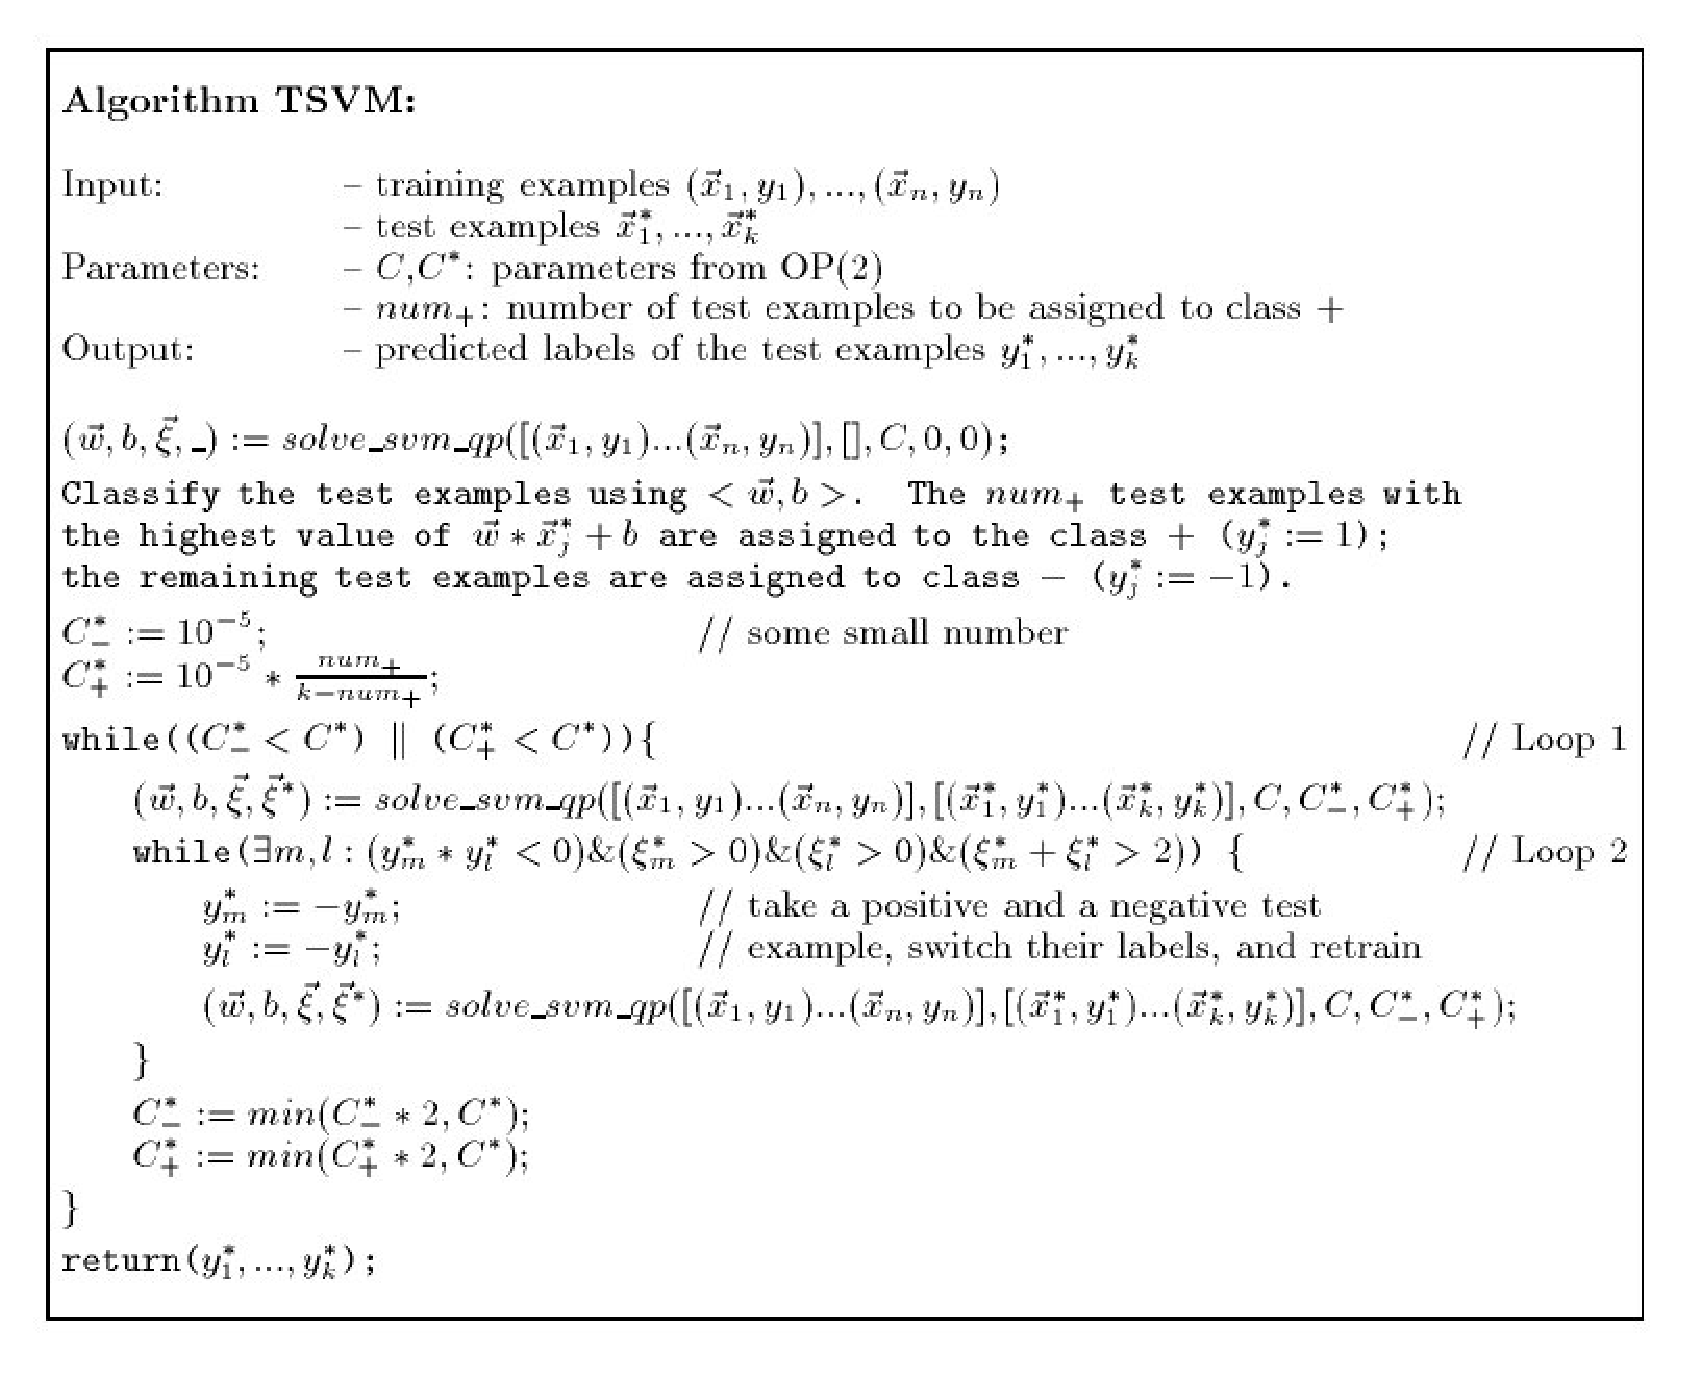
\includegraphics[scale=0.3]{images/joachims-algorithm}\label{fig:alg-tsvm}
\par\end{centering}
\caption{Algorithm for training Transductive Support Vector Machines \cite{Joachims99c}}
\end{figure}
\section{The Cascade SVM}
The Cascade SVM was described by Graf et al \cite{GrafCBDV04} and
further explored by Zhang et al \cite{ZhangZY05} and is based in
the strategy of early elimination of non-support vectors from the
training set \cite{Joachims/99a}. The Cascade SVM is a distributed
architecture where smaller optimization problems are solved independently
making them easily parallelizable. The results of this smaller problems
are then assembled in a way that is ensured that it eventually converges
to globally optimal solution.

In order to find a minimum using this approach the problem is initialized
with a number of independent smaller optimization whose results are
combined in later stages in a hierarchical fashion %as shown in figure
%\ref{fig:svm-cascade}. 

The data is split into subsets and everyone of them is evaluated for to find support vectors in the first layer,
then the results are combined two-by-two and entered as training set
for the next layer. 
%% Often a single pass through the cascade produces
%% satisfactory results and if it is not the case, that is, if solution
%% is not the global maximum, the result of the last layer is fed back
%% into the first layer, where each of the SVM of the first layer receives
%% all the support vectors and test them with fraction of his inputs
%% to check if any of them have to be incorporated into the optimization.
%% If this is not the case for all SVM of the input layer, the cascade
%% have converged otherwise it proceeds with another pass through the
%% network. The formal proof of the convergence can be found in \cite{GrafCBDV04}.
%% \begin{figure}[H]
%% \begin{centering}
%% 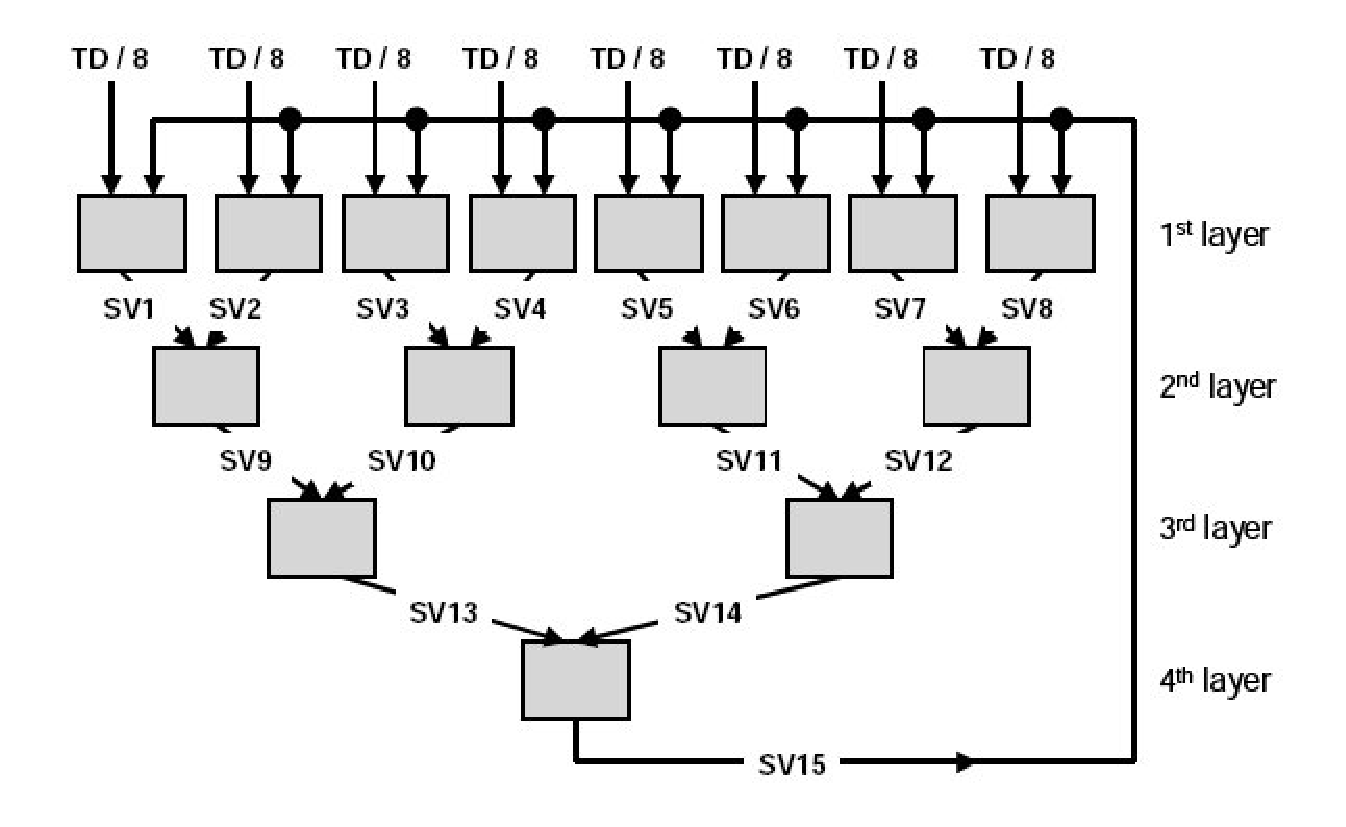
\includegraphics[scale=0.5]{images/graf-svm-cascade}
%% \par\end{centering}

%% \caption{Schematic of a Cascade architecture \cite{GrafCBDV04}}
%% \label{fig:svm-cascade}
%% \end{figure}
\subsection{Cascade Transductive SVM}

The original formulation for this cascade SVM is defined for the classical
SVM problem so it is necessary to adapt the architecture described
above in order to handle properly the TSVM formulation. 
The approach we chose was to  parallelize the more computational expensive
part of the TSVM algorithm: the \emph{solve\_svm\_qp} function which
solves the dual problem associated with formulation described in section 5 %%%%%%%%%%%%%%%%%%%%%%%%%%%% \ref{sub:Transductive-Learning-for}.
Now for each iteration of the loop the a SVM inductive problem is solved in a parallel manner. We
have two goals to achieve with this, in the first place we need to
implement an algorithm that is at least is as good as the serial (non
parallel) version and also we need to ensure a speed up of the process
through the use of the parallel architecture.
%% There are
%% at least two approach for this, the first approach is to make each
%% of theSVM in the array Transductive, using the algorithm described
%% in Figure \ref{fig:alg-tsvm}. Even if this might seem obvious ultimatly
%% the loop in each of the SVM will be run in just one processor so the
%% only possible speed up would be in terms of the number of training
%% and testing data available. Also splitting and mergin the subsets
%% might need additional modifications, despite this fact, it might be
%% interesting to vizualise the behaviour of this approach and for that
%% reason is left as a future work.
%
\begin{figure}
\begin{centering}
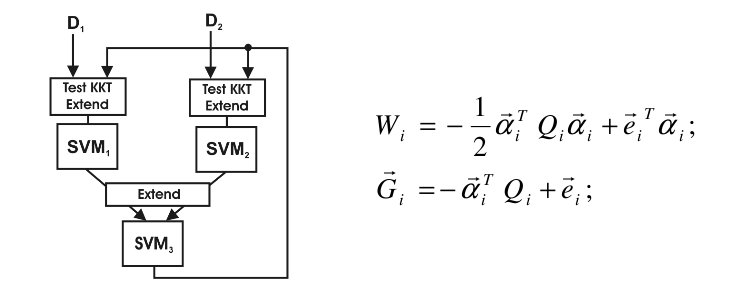
\includegraphics[scale=0.35]{images/graf-svm-cascade-of-3}\label{fig:graf-3-svm}
\par\end{centering}
\begin{centering}
\caption{A Cascade with two input sets $D_{1}$,$D_{2}$. $W_{i}$, $G_{i}$
and $Q_{i}$ are objective function, gradient, and kernel matrix,
respectively, of \noun{SVM}$_{i}$ (in vector notation); Gradients
of \noun{SVM}$_{1}$ and \noun{SVM}$_{2}$ are merged as indicated
in \ref{eq:mergin-subsets} and are entered into \noun{SVM}$_{3}$.
\cite{GrafCBDV04}}
\par\end{centering}
\end{figure}
%
\section{Merging Data Sets for the Transductive Case}

In this section it is described the procedure to merge two subsets
using as example the description in the figure \ref{fig:graf-3-svm}.
For Transductive SVM there is not practically any change besides that
when recreating creating the problem for \noun{SVM}$_{3}$ we have
to take into account two boundaries for the values of $\alpha_{i}$
instead of one: $C$ for $\{a_{1}...\alpha_{L}\}$and $C*$ for $\{a_{L+1}...\alpha_{L+U}\}$.
Also, the process of elimination of early non-support vector machine
that is made on both groups, the labeled and the unlabeled data. 

The starting point and gradient for the merged set are defined below:

\begin{eqnarray}
 & W\, & =\frac{1}{2}\left[\begin{array}{c}
\vec{\alpha_{1}}\\
\vec{\alpha}_{2}\end{array}\right]^{T}\left[\begin{array}{cc}
Q_{1} & Q_{12}\\
Q_{21} & Q_{2}\end{array}\right]\left[\begin{array}{c}
\vec{\alpha_{1}}\\
\vec{\alpha}_{2}\end{array}\right]+\left[\begin{array}{c}
\vec{e_{1}}\\
\vec{e}_{2}\end{array}\right]^{T}\left[\begin{array}{c}
\vec{\alpha_{1}}\\
\vec{\alpha}_{2}\end{array}\right]\nonumber \\
\label{eq:mergin-subsets}\\\nonumber \\ &  & \vec{G_{3}=}\left[\begin{array}{c}
\vec{\alpha_{1}}\\
\vec{\alpha}_{2}\end{array}\right]^{T}\left[\begin{array}{cc}
Q_{1} & Q_{12}\\
Q_{21} & Q_{2}\end{array}\right]+\left[\begin{array}{c}
\vec{e_{1}}\\
\vec{e}_{2}\end{array}\right]\nonumber \end{eqnarray}

With $Q_{12}=Q_{1}Q_{2}$ and $Q_{21}=Q_{2}Q_{1}$. 

%% One thing that should be noted is the error values handling. As the
%% reader can see in \ref{fig:alg-tsvm} the decision whether to swap
%% the values of the labels for each uncategorized data depends on the
%% error of the classification of that particular value but as in each
%% layer we eliminate them in the process, we have to keep a record of
%% the classification error of the eliminated unlabeled vector because
%% we are going to use in the decision of the second loop.

\section{Experiments and Results}

In this section we present the experimental results for text classification
task. The base algorithm and auxiliary routines were programmed in
Matlab 7.4%
\footnote{http://www.mathworks.com/%
} using the Matlab \emph{quadprog} function which is a convex QP solver.
In order to fully parallelize the Cascade Architecture we made use
of the Distributed Computer Tool Box which enabled us to run the algorithm
in all the cores available. For the experiments we used a Desktop
computer with Processor Intel$^{\textregistered}$ Pentium$^{\textregistered}$
Dual Core CPU 3.40GHz with 1.5 GB of RAM.

For the experiments we use a subset of the 20 Newsgroups \cite{20news}
data set found in the UCI ML Repository\cite{Asuncion+Newman:2007}.
The data set was preprocessed using English stop-words and the Porter
stemmer algorithm \cite{Porter80}. The code was written
in Ruby using an already existing implementation of the stemmer algorithm. 

The 20 Newsgroup data sets is set is a collection of approximately
20,000 newsgroup documents, partitioned evenly across 20 different
newsgroups. The collection is organized in categories ranging from computer
related topics (e.g comp.sys.ibm.pc.hardware, comp.windows.x, etc.) to
politics (talk.politics.misc,  talk.politics.guns,etc).

%% \begin{tabular}{|c|c|c|}
%% \hline 
%% %
%% \begin{minipage}[t][1\totalheight][c]{0.36\columnwidth}%
%% \begin{itemize}
%% \item comp.graphics 
%% \item comp.os.ms-windows.misc
%% \item comp.sys.ibm.pc.hardware 
%% \item comp.sys.mac.hardware 
%% \item comp.windows.x
%% \end{itemize}
%% %
%% \end{minipage} & %
%% \begin{minipage}[t][1\totalheight][c]{0.30\columnwidth}%
%% \begin{itemize}
%% \item rec.autos 
%% \item rec.motorcycles 
%% \item rec.sport.baseball 
%% \item rec.sport.hockey
%% \end{itemize}
%% %
%% \end{minipage} & %
%% \begin{minipage}[t][1\totalheight][c]{0.30\columnwidth}%
%% \begin{itemize}
%% \item sci.crypt 
%% \item sci.electronics 
%% \item sci.med sci.space
%% \end{itemize}
%% %
%% \end{minipage}\tabularnewline
%% \hline 
%% %
%% \begin{minipage}[t][1\totalheight][c]{0.25\columnwidth}%
%% \begin{itemize}
%% \item misc.forsale
%% \end{itemize}
%% %
%% \end{minipage} & %
%% \begin{minipage}[t][1\totalheight][c]{0.32\columnwidth}%
%% \begin{itemize}
%% \item talk.politics.misc 
%% \item talk.politics.guns 
%% \item talk.politics.mideast
%% \end{itemize}
%% %
%% \end{minipage} & %
%% \begin{minipage}[t][1\totalheight][c]{0.32\columnwidth}%
%% \begin{itemize}
%% \item talk.religion.misc 
%% \item alt.atheism 
%% \item soc.religion.christian
%% \end{itemize}
%% %
%% \end{minipage}\tabularnewline
%% \hline
%% \end{tabular}
\\

The data set is divided by newsgroup topics and can
be grouped into similar categories. For the experiments we define
two tasks, an {}``easy'' one and an {}``hard'' one. For the easy
task we took 1000 messages from \emph{alt.atheism }and 1000 messages
from \emph{comp.graphics}. We call this an easy task because the terms
that appear in the documents from each collection are different, so
we can expect a nearly separable problem. The hard task we chose related
news groups were is expected that the most important terms similar
for both collection. We chose c\emph{omp.sys.ibm.pc.hardware} and
\emph{comp.sys.mac.hardware }for evaluating the SVM effectiveness
and computation times with also 1000 messages from each of them. The
data was split in a training set (20\%) and testing or ulabeled set
(80\%). 
%% The unlabeled set for the TSVM was used as the testing set
%% for the classic SVM. We also made some test with fewer training data
%% but with the same amount of test data in order to visualize better
%% the goods of transductive inference when only few training data is
%% available.

As performance measure we chose $F1$ as measure of effectiveness,
we also show the values of precision and recall for the experiments.
The kernel choice for the SVM was the linear kernel which has been
reported to be effective for text categorization tasks \cite{Joachims99c,DumaisPHS98},
thanks in part to the high dimensional nature of the input vectors.
The $C$ parameter was estimated for the two sets using 5-fold cross
validation with the training set. The other parameter defined by Joachim's
algorithm is $num+$, the number of test inputs to be labeled initially
as positive, in our implementation this number is also half of the
total test set, thus ensuring the precision and recall break-even.
The choice of the parameter $C*$is done using many heuristics, however
we use the one proposed by Joachims which consists in making it equal
to $C$. %% This parameter is of great importance for the computation
%% time of the overall algorithm because the annealing used by Joachim's
%% algorithm, for that reason we wanted to improve the computation time
%% by choosing the right C{*} parameter so we tested the implementation
%% effectiveness with the original Joachim's heuristic $C=C*$.
%
%% \begin{comment}
%% and the one proposed by \cite{1248609}: $UC=LC*$ . 
%% \end{comment}
%% {}

The Cascade architecture used in the experiments were formed 3 layers
of SVM with 4 SVMs in the first 2 in the second and finally 1 in the
last layer.

Besides the categorization performance, we are interested in the computation
time, we expect that with the appropriate formulation of the parallel
architecture, reduce the impact of the computation time of the TSVM
Algorithm.
%% \subsection{Toy Experiment}
%% With the objective of prove the methods and their performance, a test
%% with few training and test samples was carried out first, the number
%% of features is also less than the full problem formulation because
%% only a fraction of these were preprocessed for this initial test.
%% For this toy experiments the hard task was performed with 200 testing
%% messages, 100 from c\emph{omp.sys.ibm.pc.hardware }labeled positive
%% and 100 from \emph{comp.sys.mac.hardware }labeled negative. The training
%% set consisted also of 200 messages with the same characteristics.
%% In these experiments (Table \ref{tab:Toy-Experiment:-comp.sys.ibm.pc.hardware})
%% the number of training samples varies for each test so we can appreciate
%% the difference in the performance of the methods. T stand for number
%% of training samples and S for number of testing samples. We can appreciate
%% that transduction algorithm perform much better than inductive when
%% few training samples, a very attractive characteristic for many real
%% problems. Even when the number of training samples is equal to the
%% number of testing samples the transductive outperforms the inductive
%% algorithm for the F measure.

%% %
%% \begin{table}[H]
%% \begin{tabular}{cc}
%% \begin{tabular}{|c|c|c|c|}
%% \hline 
%% T: 30 S: 200 & $P$  & $R$  & $F1$ \tabularnewline
%% \hline
%% \hline 
%% SVM & 0.44 & 0.8148 & 0.5714\tabularnewline
%% \hline 
%% TSVM & 0.7 & 0.7 & 0.7\tabularnewline
%% \hline 
%% TSVM Parallel & 0.7 & 0.7 & 0.7\tabularnewline
%% \hline
%% \end{tabular} & \begin{tabular}{|c|c|c|c|}
%% \hline 
%% T: 100 S: 200 & $P$  & $R$  & $F1$ \tabularnewline
%% \hline
%% \hline 
%% SVM & 0.94 & 0.7581 & 0.8393\tabularnewline
%% \hline 
%% TSVM & 0.84 & 0.84 & 0.84\tabularnewline
%% \hline 
%% TSVM Parallel & 0.84 & 0.84 & 0.84\tabularnewline
%% \hline
%% \end{tabular}\tabularnewline
%%  & \tabularnewline
%% \begin{tabular}{|c|c|c|c|}
%% \hline 
%% T: 200 S:200 & $P$  & $R$  & $F1$ \tabularnewline
%% \hline
%% \hline 
%% SVM & 0.94 & 0.7666 & 0.8624\tabularnewline
%% \hline 
%% TSVM & 0.87 & 0.87 & 0.87\tabularnewline
%% \hline 
%% TSVM Parallel & 0.87 & 0.87 & 0.87\tabularnewline
%% \hline
%% \end{tabular} & \tabularnewline
%% \end{tabular} 
%% \caption{Small Scale Experiment: \emph{comp.sys.ibm.pc.hardware} and\emph{
%% comp.sys.mac.hardware} with 200 messages from each newsgroup. \label{tab:Toy-Experiment:-comp.sys.ibm.pc.hardware}}
%% \end{table}
\subsection{Easy Task}

As mentioned above the easy task is an experiment were is expected
a linear separable problem formed by messages from newsgroups with
very disjoint topics. The number of features for each vector was 30854,
a high dimensional problem the with the parameter C = 10 from the
5-fold cross validation. Table \ref{tab:Easy-Task:comp.graphics-and}
shows the results of the experiments. 

%
\begin{table}
\begin{longtable}
%% \begin{tabular}{|c|c|c|c|c|c||c|}
%% \hline 
%%  & \#Labeled & \#Unlabeled & $P$  & $R$  & $F1$  & Time (min)\tabularnewline
%% \hline
%% \hline 
%% SVM & 200 & N/A & 0.9245 & 1.0 & 0.9608 & 0.0137\tabularnewline
%% \hline 
%% TSVM & 200 & 200 & 0.9847 & 0.9847 & 0.9847 & 10.2205\tabularnewline
%% \hline 
%% TSVM Parallel & 200 & 200 & 0.9847 & 0.9847 & 0.9847 & \textcolor{red}{7.2050}\tabularnewline
%% \hline
%% \end{tabular} \\
\begin{tabular}{|c|c|c|c|c|c||c|}
\hline
 & \#Train\ \ \ \ & \#Unlabeled & $P$  & $R$  & $F1$  & Time (min)\tabularnewline
\hline 
SVM & 200 & N/A & 0.9384 & 1 & 0.9682 & 0.0135\tabularnewline
\hline 
TSVM & 200 & 400 & 0.9823 & 0.9823 & 0.9823 & 44.4103\tabularnewline
\hline 
TSVM Parallel & 200 & 400 & 0.9823 & 0.9823 & 0.9823 & 15.3406\tabularnewline
\hline
\end{tabular}\\
\tabularnewline
\tabularnewline
\begin{tabular}{|c|c|c|c|c|c||c|}
\hline 
 & \#Train\ \ \ \ & \#Unlabeled & $P$  & $R$  & $F1$  & Time (min)\tabularnewline
\hline 
SVM & 100 & N/A & 0.9062 & 1 & 0.9508 & 0.0135\tabularnewline
\hline 
TSVM & 100 & 400 & 0.9823 & 0.9823 & 0.9823 & 32.1135\tabularnewline
\hline 
TSVM Parallel & 100 & 400 & 0.9823 & 0.9823 & 0.9823 & \textbf{11.0953}\tabularnewline
\hline
\end{tabular} \\
\tabularnewline
\tabularnewline
\begin{tabular}{|c|c|c|c|c|c||c|}
\hline 
 & \#Train\ \ \ \ & \#Unlabeled & $P$  & $R$  & $F1$  & Time (min)\tabularnewline
\hline
\hline 
SVM & 100 & N/A & 0.9975 & 0.8957 & 0.9438 & 0.0135\tabularnewline
\hline 
TSVM & 100 & 800 & 0.9798 & 0.9798 & 0.9798 & 214.2297\tabularnewline
\hline 
TSVM Parallel & 100 & 800 & 0.9798 & 0.9798 & 0.9798 & 	\textbf{68.4745}\tabularnewline
\hline
\end{tabular}\\
\tabularnewline
\tabularnewline
\begin{tabular}{|c|c|c|c|c|c||c|}
\hline 
 & \#Train\ \ \ \ & \#Unlabeled & $P$  & $R$  & $F1$  & Time (min)\tabularnewline
\hline
\hline 
SVM & 100 & 0 & 0.8966 & 0.9975 & 0.9444 & 0.0135\tabularnewline
\hline 
TSVM & 100 & 1600 & 0.9800 & 0.9800 & 0.9800 & 278.3236%
\tabularnewline
\hline 
TSVM Parallel & 100 & 1600 & 0.9800 & 0.9800 & 0.9800 & \textbf{41.53950}\tabularnewline
\hline
\end{tabular}\tabularnewline
\end{longtable}

\caption{The {}``Easy'' Task:\emph{ comp.graphics} and \emph{alt.atheism}.
Using C=10 \label{tab:Easy-Task:comp.graphics-and} }

\end{table}

We can notice how the classical SVM algorithm is always faster that
the Transductive implementation and for this specific problem, which
is expected to be almost linear separable, with few unlabeled data
the classification performance is very similar, while the difference
in speed of the algorithm is really huge. However when the training
data decreases and more there is more unlabeled data the differences
in classification performance begin to be more noticeable, even with
this {}``easy'' problem. Regarding the speed, is obvious by the
results that that the standard SVC algorithm is by far faster than
its transductive counterparts, therefore we are going to discuss the
differences between the transductive and its parallel version. For
this problem, the classification performance of the transductive algorithms
were the same, thus one of the objectives was accomplished, to maintain
the same classification performance while performing the tasks in
parallel. Of course, the gains of the parallel approach and the early
eliminations of non-support vectors are devised in the time used for
the calculations on the Transductive SVM problem.
%%  One thing that can
%% be noticed in the tables is that the parallel version of the algorithm
%% no necessarily is slower when facing much more data, this is due to
%% the process of early elimination of non-support vector and it may
%% happen that with much more data more non-support vectors are eliminated
%% in proportion with the amount of unlabeled data, making the whole
%% process faster. This particular property can be really appealing when
%% working with larger datasets, of course it will depend entirely on
%% the dataset.

\subsection{Hard Task}

This is task is formed from 2000 messages from the categories of \emph{comp.sys.ibm.pc.hardware}
and\emph{ comp.sys.mac.hardware} which have many equal terms thus
making it a possible not linearly separable problem. The number of
features extracted for this problem is 26997. The parameter choice
for C = 9 and was taken from the same 5-fold cross-validation with
the available training data.

%
\begin{table}
\begin{longtable}
\begin{tabular}{|c|c|c|c|c|c||c|}
\hline
 & \#Train & \#Unlabeled & $P$  & $R$  & $F1$  & Time (min)\tabularnewline
\hline 
SVM & 100 & N/A & 0.7400 & 0.8916 & 0.8087 & 0.0025\tabularnewline
\hline 
TSVM & 100 & 200 & 0.8600 & 0.8600 & 0.8600 & 1.5370\tabularnewline
\hline 
TSVM Parallel & 100 & 200 & 0.8700 & 0.8700 & 0.8700 & 1.4863\tabularnewline
\hline
\end{tabular} \\
\tabularnewline
\tabularnewline
\begin{tabular}{|c|c|c|c|c|c||c|}
\hline 
 & \#Train & \#Unlabeled & $P$  & $R$  & $F1$  & Time (min)\tabularnewline
\hline 
SVM & 100 & N/A & 0.8830 & 0.7550 & 0.8140 & 0.0025\tabularnewline
\hline 
TSVM & 100 & 400 & 0.8550 & 0.8550 & 0.8550 & 6.0628\tabularnewline
\hline 
TSVM Parallel & 100 & 400 & 0.8550 & 0.8550 & 0.8550 & 4.3323\tabularnewline
\hline
\end{tabular} \\
\tabularnewline
\tabularnewline
\begin{tabular}{|c|c|c|c|c|c||c|}
\hline 
 & \#Train & \#Unlabeled & $P$  & $R$  & $F1$  & Time (min)\tabularnewline
\hline
\hline 
SVM & 100 & N/A & 0.7350 & 0.8724 & 0.7978 & 0.0025\tabularnewline
\hline 
TSVM & 100 & 800 & 0.8200 & 0.8200 & 0.8200 & 31.0015\tabularnewline
\hline 
TSVM Parallel & 100 & 800 & 0.8200 & 0.8200 & 0.8200 & 19.5472\tabularnewline
\hline
\end{tabular} \\
\tabularnewline
\tabularnewline
\begin{tabular}{|c|c|c|c|c|c||c|}
\hline 
 & \#Train & \#Unlabeled & $P$  & $R$  & $F1$  & Time (min)\tabularnewline
\hline
\hline 
SVM & 100 & 0 & 0.7362 & 0.8624 & 0.7943 & 0.0135\tabularnewline
\hline 
TSVM & 100 & 1600 & 0.8187 & 0.8187 & 0.8187 & 221.5013\tabularnewline
\hline 
TSVM Parallel & 100 & 1600 & 0.8187 & 0.8187 & 0.8187 & 86.1924\tabularnewline
\hline
\end{tabular}\tabularnewline
\tabularnewline
\tabularnewline
\tabularnewline
\end{longtable}

\caption{The {}``Hard'' Task:\emph{ }of \emph{comp.sys.ibm.pc.hardware} and\emph{
comp.sys.mac.hardware}. Using C=9 \label{tab:Hard-Task:comp.graphics-and} }

\end{table}

As expected, the TSVM performed better than the classic linear SVM,
however due to the nature of the data, the classification performance
difference between the two the TSVM and the SVM was not really substantial.
Another thing to notice is that this example is somewhat counter-intuitive,
because you could expect that for more training data available the
difference between the classification performance between the classical
and the transductive SVM would increase. However the opposite happened,
when more training data was available, the difference between their
performance decreased. Another result of the experiment, that surprised
us but we knew it could happen was the for the 100-200 setup the transductive
parallel SVM had a little bit more classification performance than
the non-parallel version. Even with this particularities in general
terms the expected occurred, the classification performance of the
transductive setting was higher than the inductive one, and the parallel
version of the TSVM run almost 3 times faster than the non transductive
one.

\section{Conclusions and Future Directions}

In this work we have implemented a parallel version of TSVM as described
by Joachims' \cite{Joachims99c}, an approach that because its annealing
heuristics requires many iterations solving a similar problems. Our
approach, in order to speed up the process, was to parallelize the
SVM solver function using a Cascade architecture. We have shown that
this approach speed up the process 2 to 7 times using just one dual
core processor. This architecture scales very well, therefore is expected
that, with more processors available the the speed gains will be even
more noticeable. In addition, more layers in the  basic architecture could
help in the improvement of the computation time. 

From the data tables one could argue that the classification performance
gains for using TSVM does not worth the computation time spent even
with this parallel approach. However this last statement is in someway
subjective, as the trade-off between speed and classification performance
depends in nature of the problem, it would be possible that we would
prefer more classification performance at cost of computation time.
Also, if more and more processors/cores available (as it is the actual
trend) the speed gains could be much more noticeable. 

Regarding the classification performance of the TSVM algorithm we
noticed something particular, the best C for the C{*} for the transductive
setting does not generally match in the sense that the best C parameter
for the inductive problem does not produce the best classification
performance in the transductive problem for the given set of data.
However, we have chosen the parameter that works best for the inductive
setting.

It is truth that more optimization strategies have to be developed
in order to make this algorithm really usable in real world situation.
Now, with a parallel and scalable version of the transductive algorithm
a series of strategies could be explored in order to further optimize
the computation time, however the implementation of such strategies
is outside the scope of this work.
 % and are mentioned here as a possible
%future work.

%% Maybe the most obvious approach is that given that the data is split
%% in equal parts (subsets), and per each iteration only one of the parts
%% is modified (i the labels of two of the entries) there is not need
%% recalculate the other parts of the n and they can be reused. For example
%% in our particular case, we calculated 7 distinct SVM problems (as
%% our architecture o 3 layers t in 4-2-1 e respectively), using caching
%% we wold only need to calculate all of them once at the r and then
%% only when a pair of of vector fell of different SVM problem. For the
%% most of the iterations we would only need to calculate 3 problems. 

%% Another strategy would be try new improved heuristics as described
%% by Collobert et al \cite{citeulike:935557|Collobert2002} and modifying
%% in Joachims' TSVM by reducing iteration in the cycles or interchanging
%% more labels per iteration. This last is important because the annealing
%% heuristic used by Joachim's TSVM is source of the elevated computation
%% time.

%% A good thing about this approach is that any improvement to the SVM
%% formulation can be directly applied to the SVM, for example the technique
%% of Zanghirati et al. \cite{782654}could be applied to each one of
%% the SVM solvers in order to have multilevel parallelization, further
%% improving the computation performance.

\bibliography{biblio}{}
\bibliographystyle{plain}

%
% ---- Bibliography ----
%
%% \begin{thebibliography}{5}
%% %
%% \bibitem {clar:eke}
%% Clarke, F., Ekeland, I.:
%% Nonlinear oscillations and
%% boundary-value problems for Hamiltonian systems.
%% Arch. Rat. Mech. Anal. {\bf 78} (1982) 315--333
%% %
%% \bibitem {clar:eke:2}
%% Clarke, F., Ekeland, I.:
%% Solutions p\'{e}riodiques, du
%% p\'{e}riode donn\'{e}e, des \'{e}quations hamiltoniennes.
%% Note CRAS Paris {\bf 287} (1978) 1013--1015
%% %
%% \bibitem {mich:tar}
%% Michalek, R., Tarantello, G.:
%% Subharmonic solutions with prescribed minimal
%% period for nonautonomous Hamiltonian systems.
%% J. Diff. Eq. {\bf 72} (1988) 28--55
%% %
%% \bibitem {tar}
%% Tarantello, G.:
%% Subharmonic solutions for Hamiltonian
%% systems via a $\bbbz_{p}$ pseudoindex theory.
%% Annali di Matematica Pura (to appear)
%% %
%% \bibitem {rab}
%% Rabinowitz, P.:
%% On subharmonic solutions of a Hamiltonian system.
%% Comm. Pure Appl. Math. {\bf 33} (1980) 609--633
%% \end{thebibliography}
%
\end{document}
